\section{Design}\label{sec:design}
Naively vectorizing arbitrary arithmetic circuits looks a lot like SLP: we start by serializing the circuit into a sequence of scalar three-address instructions.
At each step, we look at all available scalar instructions (i.e. instructions whose source operands have all already been scheduled), pick the largest set with the same operation, and schedule them together.
The problem with this naive strategy is it makes no guarantees about values being computed and used on the same lane; in other words, it incurs arbitrarily many shuffles to make the computation line up on the correct lanes.
Unlike in normal vectorization, where applying arbitrary permutations to the lanes is relatively cheap, in FHE we are only allowed to rotate the entire vector by a fixed number of slots, and this rotation operation is expensive.
Hence, the cost of bookkeeping quickly outweighs whatever benefit we might get from vectorization, making this approach not worth it.

In effect, when trying to compute an efficient vector schedule \raghav{Terminology things once again: I need a word for ``vertical alignment'' that isn't ``schedule'', since I want to use ``schedule'' to refer to the combination of vertical {\em and} horizontal alignment\dots} for an FHE program, we have two optimization problems to solve: instruction scheduling, and data layout.
Optimizing only for instruction scheduling essentially gives us the SLP approach: aggressively pack together isomorphic instructions without worrying about the incurred data movement overhead.
Optimizing for data layout places us on the other end of the spectrum: to avoid having to do any rotates, we must place each connected component of the circuit on a single lane, effectively precluding any vectorization and forcing us to execute everything as scalar operations.

One of our key insights is that these two problems are highly related, so we have to solve these {\em simultaneously} rather than independently, effectively attempting to choose an optimal point in the tradeoff space between the two ends of the spectrum.
In the following sections, we lay out the exact optimization problem as well as how we search for a solution. 

\subsection{Overview}
The vector {\em pre-schedule}\footnote{This structure is referred to as a {\em pre-schedule} to distinguish it from the actual vector schedule, which explicitly computes an alignment for sequences of instructions at the same level. \raghav{does this make sense?}} is a labeled quotient of the original circuit graph, where each vertex represents a connected subgraph, and is labeled with an integer representing the lane the subgraph gets placed on, satisfying the condition that no two vertices at the same height are labeled by the same lane.
The pre-schedule is naturally bi-graded into {\em epochs}, or groups of (independent) vertices at the same height which get packed together into a single sequence of vector instructions requiring no data movement, as well as {\em columns}, groups of vertices assigned to the same lane representing computation that happens in a single thread with no internal vectorization.\raghav{There's something interesting to say here about how the circuit is filtered by height, and the vertical grading is actually the grading associated to this filtration, and the ``quotient'' is what you get when you mod out by the kernel of the lane assignment at each degree (which in fact is where that uniqueness condition from before comes from).}
Note that the uniqueness condition stated above means that each vertex of the quotient graph can be uniquely identified by its epoch and column (although the converse in general does not hold, since its possible to have a column that does not contain every epoch and vice-versa).

It turns out that both of our extremes from earlier can be realized in this model.
Aggressively vectorizing SLP-style can be recovered by assigning a trivial subcircuit to each vertex of the quotient, and simply enumerating lanes across epochs.
On the other end of the spectrum, we could instead quotient the circuit into the discrete graph of its connected components and assign each discrete vertex an arbitrary lane; since this graph has no edges it requires no rotations, but also precludes any vectorization within connected components.

Finding a good pre-schedule then requires us to first compute a ``good'' quotient that trades off between these extremes, together with a lane assignment that somehow maximizes our ability to vectorize without incurring too many rotations.
The next section discusses what makes one graph quotient ``better'' than another, and exactly how these tradeoffs are quantified.

\subsection{Cost Model}\label{sec:cost-model}
The cost of a particular pre-schedule comes from two places: the number of rotations we have to perform, and the amount we've ``given up'' on vectorizing.
\subsubsection*{Rotations}
Given a vector schedule, each {\em cross-lane arc} in the graph (an arc connecting vertices of different lanes) represents a rotation that must be performed to align an output from the tail of the arc to where it gets used at the head.
However, determining the rotation overhead is not as simple as counting these arcs.
Consider the case where instructions $A$ and $B$ are operands to instructions $A'$ and $B'$, respectively.
If $A$ and $B$ are assigned lanes $n$ and $m$, $A'$ and $B'$ are assigned $n+k$ and $m+k$, and $A$ and $B$ end up packed together in the same vector instruction, the two separate data movement operations required for the $A\to A'$ arc and the $B\to B'$ can actually be instantiated with a single rotation by $k$ slots of the $[A, B]$ vector (In fact, taking advantage of this fact is the main way we can optimize data layout to require fewer total rotates). 
To compute the {\em actual} number of rotations required for a particular schedule, we instead proceed epoch-by-epoch. 
For each epoch, we look at all cross-lane arc with tails in that epoch, and compute its {\em span} (the required rotation amount) by subtracting the lane at the tail from the lane at the head.
The rotation cost for that epoch is then just the number of distinct rotation amounts\footnote{In practice, this underestimates the number of rotation instructions, since a given epoch might be packed into a sequence of multiple vector operations, so rotations of the same amount might not be carried out by a single instruction. This is addressed in Section~\ref{sec:optimality-tradeoffs}}.
For example, if a particular epoch has five cross-lane arcs, of which three represent a rotation of $-1$ and two represent a rotation of $6$, its rotation cost is $2$.
It follows that the total rotation cost of a schedule is the sum of the rotation costs of each epoch.

\subsubsection*{Vectorizability}
Taking successive quotients of the circuit reduces the total number of edges, and by extension, reduces the number of rotates that might be required; however, it also precludes any vectorization within the collapsed subcircuits.
To account for this, and to prevent the optimal schedule from being the trivial one described above, we need a way of quantifying the amount of vectorization we're ``giving up'' with each quotient.

Unfortunately, directly computing the opportunity cost is very messy: the amount of vectorization we give up by identifying a set of vertices is not a property local to the vertices, but rather requires us to look globally at {\em all possible vertices} in those epochs, to see which vectorization opportunities are no longer available after the identification.
Instead, we use an estimated {\em schedule height} as a proxy, with the justification being that giving up a lot of vectorization generally results in taller, less efficient final schedules. \raghav{Is it enough to say this? Or do I need to justify it further? Or should I remove these paragraphs entirely and just directly describe the schedule height computation?}

The schedule height computation once again proceeds epoch-by-epoch.
For each epoch, we estimate the minimum number of vector instructions required after packing by taking the maximum number of each type of operation across all the subcircuits associated to the vertices in that epoch\footnote{Once again, this is an underestimate of the actual height when the schedule is fully realized, since it doesn't take into account any dependences between the instructions. This is addressed in Section~\ref{sec:optimality-tradeoffs}}.
For example, consider an epoch with two vertices, one with 3 adds and 2 multiplies, and one with 2 adds and 4 multiplies.
The estimated height for this epoch would be 3 adds and 4 multiplies.

\subsubsection*{Overall Cost}
The analysis presented above computes an estimate for the number of each type of instruction in the generated vector program.
The final cost used a linear combination of all of these, with weights determined empirically by how expensive each instruction type is relative to the rest.
In our implementation, we scale rotates and multiplies by $1$, and addition and subtraction by $0.1$. \raghav{Should this last sentence go here, or in implementation? Or both?}

\subsection{Schedule Search}\label{sec:schedule-search}
Given a cost model, we use a two-layer optimization strategy to produce a schedule that has good packing properties without incurring too much data movement overhead.
\subsubsection*{Determining lane placement}
\begin{algorithm}
    \SetKwFunction{placelanes}{PlaceLanes}
    \SetKwFunction{naive}{InitialPlacement}
    \SetKwFunction{permute}{GenerateCandidate}
    \SetKwFunction{cost}{Cost}
    \SetKwFunction{accept}{Accept}
    
    \SetKwProg{algo}{Algorithm}{}{}
    \SetKwProg{proc}{Procedure}{}{}

    \algo{\placelanes{graph}}{
        $lanes \gets \naive{graph}$\;
        $T \gets T_0$\;
        $cost \gets \cost{lanes, graph}$\;
        \For{$i = 1 : N$}{
            $T \gets T / (1 + \beta T)$\;
            $candidate \gets \permute{lanes, graph}$\;
            $cost' \gets \cost{candidate, graph}$\;
            \If{$\accept{cost, cost', T}$}{
                $lanes\gets candidate$\;
                $cost \gets cost'$\;
            }
        }
        \Return{lanes, cost}
    }
    \proc{\cost{lanes, graph}}{
        $rotations[*] \gets \emptyset$\;
        \ForEach{$(u\to v) \in graph$}{
            \If{$lanes[u]\neq lanes[v]$}{
                $rotations[u.epoch] \gets rotations[u.epoch]\cup \{lanes[v] - lanes[u]\}$\;
            }
        }
        $instrs[*]\gets 0$\;
        \ForEach{$epoch \in graph$}{
            \ForEach{$opcode$}{
                $instr[opcode] \gets instr[opcode] + \max\limits_{col}count(epoch, col, opcode)$\;
            }
        }
        \Return{$w_R\times\sum\limits_{ep} rotations[ep] + \sum\limits_{op} w_{op}\times instrs[op]$}
    }
    \caption{Lane placement}\label{alg:lane-placement}
    
\end{algorithm}
The inner layer uses simulated annealing to find an optimal lane assignment for a given quotient graph.
The initial assignment is the naive one given by simply enumerating the vertices at each epoch.
At each step of the algorithm, we generate a candidate solution by randomly choosing two columns and a subset of the epochs in them to swap, maintaining the uniqueness condition of the schedule.
If the overall cost (as described in Section~\ref{sec:cost-model})\footnote{We could have chosen to only look at the rotation cost of each solution, but considering both costs helps prioritize lane placements with a heterogeneity of instruction types within each lane} of the candidate solution is lower than the original cost, it is accepted, and used as the starting point for the next round.
If the candidate solution cost is {\em higher} than the original cost, it is accepted with a probability that varies negatively with the difference in cost, and is generally smaller in later rounds than in earlier rounds\footnote{We use a slow cooling schedule with initial temperature $T_0=50$ and cooling parameter $\beta=10^{-3}$. The probability of accepting a move that increases the cost by $\Delta_c$ is $e^{-\Delta_c/T}$. The annealing is run for $20$k rounds.}.
After a fixed number of rounds have elapsed (see footnote), this algorithm returns the best solution found so far.

\subsubsection*{Computing optimal circuit quotient}
\begin{algorithm}
    \SetKwFunction{quotient}{ComputeQuotient}
    \SetKwFunction{placelanes}{PlaceLanes}
    \SetKwFunction{accept}{Accept}
    \SetKwFunction{contract}{ContractEdge}
    \SetKwFunction{condensation}{Condensation}
    \SetKwFunction{cross}{CrossArcs}
    \SetKwFunction{enq}{Enqueue}
    \SetKwFunction{deq}{Dequeue}

    \SetKwProg{algo}{Algorithm}{}{}

    \algo{\quotient{graph}}{
        $lanes, cost \gets \placelanes{graph}$\;
        $best \gets lanes, graph$\;
        $bestcost \gets cost$\;
        $pqueue\gets []$\;
        $\enq{pqueue, (graph, lanes), cost}$\;
        \For{$i = 1 : N$}{
            $graph, lanes \gets \deq(pqueue)$\;
            \If{$arc \samplefrom \cross{graph}$}{
                $candidate \gets \condensation{\contract{graph, arc}}$\;
                $lanes', cost' \gets \placelanes{candidate}$\;
                $\enq{pqueue, (candidate, lanes'), cost'}$\;
                \If{$cost' < bestcost$}{
                    $best \gets lanes', candidate$\;
                }
                $\enq{pqueue, (graph, lanes), cost}$\;
            }
        }
        \Return{best}
    }
    \caption{Computing a good circuit quotient}\label{alg:circuit-quotient}
\end{algorithm}
The outer layer searches the space of quotients for a graph that admits a good lane placement without giving up too much vectorizability.
Here, we use a priority queue to implement a simple best-first search.
Each graph in the queue is assumed to already be equipped with an optimal lane placement, via the algorithm described above.
At each step, a graph is dequeued, and a new candidate solution is generated by looking at its set of cross-lane arcs and choosing one to contract.
The contracted graph may not be acyclic, so we first mod out by all cycles before running the lane placement algorithm again.
The candidate solution is then enqueued with a priority based on its cost from the annealed lane placement.
If there are more available arcs to contract, the original graph is enqueued again.

After a fixed number of rounds have elapsed, or once the queue is empty, the algorithm terminates and returns the best graph.
Since each step of this algorithm involves an expensive call to the lane placement procedure, this runs for a much smaller number of rounds, usually between 150 and 200.
In practice, this is enough to find highly efficient schedules.





% \raghav{Do I need to explain what simulated annealing is from scratch, or can I just describe the two-layer approach?}

% \subsection{Selecting Vectorizable Subexpressions}\label{sec:selecting-subexpressions}

% %\raghav{This sounds kind of convoluted, I wonder if there's a shorter way to say it}
% The unit of vectorization in \system is a \textit{subexpression}: a backwards slice through the circuit rooted at a particular operation and extending back all the way to the input---in other words, a subtree rooted at a particular operation. In the circuit of Figure~\ref{fig:small-expr-circuit}, there are five subexpressions, rooted at each of the five arithmetic operations. Note that this means that subexpressions are not necessarily disjoint: one can be contained within another, or, in the case of circuits that are DAGs, two subexpression may share common sub-subexpressions.

% \system's goal is to find several independent (disjoint) subexpressions that have some commonality---similar structure that allows one or more of the operations within those subexpressions to be performed as a single vector operation. By considering entire subexpressions to group together, rather than individual operations, \system can place all the operations of a given subexpression into a single lane, avoiding rotations for all of them.

% \system finds a group of similar subexpressions and schedules them together into a vector {\em epoch}. It then quotients the subexpressions out of the circuit, meaning that several subtrees in the original circuit get collapsed into single nodes that represent the output of that subtree. For example, after quotienting out the two shaded subexpressions in Figure~\ref{fig:small-expr-circuit}, what remains is a tree with a single multiplication operation, whose operands are the results of the two shaded subexpresions. \system then repeats the process for the remainder circuit. Algorithm~\ref{alg:find-epochs} shows this process formally. 

% The key questions \system must address are: (i) How does it determine how similar two subexpressions are? (ii) How does it determine which subexpressions to place into an epoch?

% \subsubsection*{Measuring subexpression vectorizability}
% We want to measure how well the instruction sequences corresponding to two arbitrary expressions line up.
% Given an arithmetic circuit, we can inductively compute the structural similarity between every pair $(t_1, t_2)$ of independent subcircuits (two circuits are independent if they have no overlap) as follows: %\milind{Hmmm... I guess here we're pretty tied to the expression tree representation of circuits, so forget what I said earlier about thinking in terms of dependence graphs. Maybe make clear in section 2.1.2 that we'll think of circuits as expression forests or expression DAGs, where leaves are data and interior nodes are operations}

% \begin{align*}
%     sim(t_1, var) &= 0\\
%     sim(var, t_2) &= 0\\
%     sim(t_1, t_2) &= \max \begin{cases}
%         sim(t_1.L, t_2)\\
%         sim(t_1.R, t_2)\\
%         sim(t_1, t_2.L)\\
%         sim(t_1, t_2.R)\\
%         sim(t_1.L, t_2.L) + sim(t_1.R, t_2.R) + b\\
%         sim(t_1.L, t_2.R) + sim(t_1.R, t_2.L) + b
%     \end{cases}
% \end{align*}
% where $t_i.L$ and $t_i.R$ represent the left and right subcircuits\footnote{If $t_i$ is a DAG but not a tree, it is possible that $t_i.L = t_i.R$. This is fine.} of $t_i$, $var$ represents a leaf node, and $b = 1$ if $t_1.op = t_2.op$ and $0$ otherwise.

% Intuitively, this formula says that the similarity between any tree and a leaf node (which is an input variable) is $0$.
% To compute the similarity between two trees, we consider the best of all six possible ways of aligning them, adding to the similarity score if the roots align with the same operation. %\raghav{Intuitive enough? I considered writing out the six possible ways of aligning them but that's what I had before and it sounded even more confusing.}\milind{I think it's OK.}

% For example, in the circuit from Figure~\ref{fig:small-expr-circuit}, we have a similarity score of $2$ between $(ab + c)$ and $(xy + z)$. %\raghav{Should I step through the induction here to show why that's the case?}\milind{If there's space, sure...}

% % The base case is comparing any tree to a leaf node (a single variable with no operations), in which case the similarity is $0$, as there are no operations that can be packed together.

% % In the inductive case of two nontrivial trees, there are six ways they could be lined up: \raghav{TODO: diagram}
% % Either root could be lined up with either child of the other tree in four ways. 
% % Or, the two roots could line up, giving two ways for their children to line up (left with left and right with right, or left with right and right with left).
% % In the first four cases, the similarity score of the two trees is the similarity score of the alignment. 
% % In the last two cases, the similarity score of the two trees is the sum of the scores of the aligned children, plus a 1 if the roots have the same operation.
% % The final similarity score of the two trees is the maximum possible score out of all six cases. 
% % \raghav{This makes no sense even to me, and I was looking at the code when I wrote this.}\milind{Actually, now that I think about it, maybe write this as a set of recurrence relations, a la smith waterman}

% \subsubsection*{Choosing maximally vectorizable sets}%\raghav{TODO: add a running example $(ab+c)(xy+z)$}
% \begin{algorithm}
%     \SetKwFunction{vecgraph}{GetVectorizabilityGraph}
%     \SetKwFunction{getclique}{MaxClique}
%     \SetKwFunction{removenodes}{RemoveNodes}
%     \SetKwFunction{updateweights}{UpdateEdgeWeights}
%     \SetKwFunction{epochs}{FindEpochs}
%     \SetKwFunction{subexprs}{SubExprs}
%     \SetKwFunction{similarity}{Similarity}

%     \SetKw{Continue}{continue}

%     \SetKwProg{proc}{Procedure}{}{}
%     \SetKwProg{algo}{Algorithm}{}{}

%     \algo{\epochs{expr}}{
%         $graph \gets \vecgraph{expr}$\;
%         $epochs \gets []$\;
%         \While{clique $\gets$ \getclique{graph}}{
%             \removenodes{graph, clique}\;
%             \updateweights{graph, clique}\;
%             $epochs$.append($clique$)
%         }
%         \Return{epochs}\;
%     }

%     \proc{\vecgraph{expr}}{
%         $V \gets \emptyset$\;
%         $E \gets \emptyset$\;
%         $weights \gets \emptyset$\;
%         \ForEach{$e, e' \in $ \subexprs{expr}, $e\cap e' = \emptyset$}{
%             $V \gets V \cup \{e, e'\}$\;
%             $E \gets E \cup \{(e, e')\}$\;
%             $weights[e, e'] \gets \similarity(e, e')$\;
%         }
%         \Return{V, E, weights}
%     }
%     \caption{Identifying vectorizable epochs}\label{alg:find-epochs}
% \end{algorithm}

% %Not every pair of subexpressions is eligible to be vectorized together, since they have to be independent of each other: if one subexpression is contained in another, or two subexpressions share a common subcircuit, they must be handled separately.
% Information about which subexpressions are independent of one another can be encoded in an undirected {\em vectorizability graph}, where each subexpression is a vertex, and there is an edge between two vertices if the corresponding subexpressions are independent (and thus vectorizable). Note that there are as many vertices in this graph as there are operations in the arithmetic circuit (each operation is the root of a subexpression), and that a {\em specific} operation may be part of more than one subexpression (those subexpressions are necessarily {\em not} independent).

% Cliques in this graph correspond exactly to sets of expressions that can all be vectorized together. 
% We can further label each edge with the similarity score of the two subexpressions it connects.
% Since each similarity score roughly corresponds to the number of instructions that could be packed together, the total weight of a clique represents the total number of operations we save by vectorizing together all the subexpressions contained within. 
% There is a subtlety here: if we just take the largest clique in the graph, we do get to vectorize a lot of expressions, but this also potentially incurs more rotates down the line.
% To account for this, we have the choice\footnote{The details of how we make this choice are discussed in Section~\ref{sec:penalizing-rotates}} to penalize larger cliques by, for example, subtracting a fixed amount from every edge.
% % There is a subtlety here: we don't just want to take the largest clique in the graph, since this means vectorizing a lot of expressions, which will likely incur several rotates down the line. 
% % To account for this, we subtract a fixed \milind{Not fixed---based on size of the clique} amount from the weight of each edge; this penalizes large cliques, and ensures that we prioritize finding small cliques of highly vectorizable expressions to avoid doing too many rotations. 
% %\milind{Be more vague about this subtraction bit, since we maybe don't do it exactly like that anymore :-) You can add something in implementation that's specifically about the weighting...}\raghav{Is that better now? Or should I not be saying subtract at all}
% %\milind{seems fine}
% % By simply subtracting a fixed amount from the weight of each edge we can penalize large cliques which would incur a much higher rotation overhead, unless the vectorizability of the clique is high enough to be worth it. \milind{Rephrase this: start by explaining why you don't want to just take super big cliques -- it doesn't take into account rotation -- and then explain how you adjust the weights to account for this}
% The problem of finding a set of subexpressions to vectorize together reduces to finding a maximal weight clique in this graph, which is easily packaged off to an SMT solver.

% This approach greedily selects a set of expressions to vectorize, which amounts to scheduling the first {\em epoch} of the program. We want to repeat the process until the entire program has been scheduled.
% Repeating the process requires some extra work: whenever a set of subexpressions is selected, each one needs to be ``quotiented out'' of the original program (i.e. collapsed to a new leaf node in the circuit).
% Doing so requires that we make two changes to the vectorizability graph:
% \begin{enumerate}
%     \item All the nodes that were cut out of the circuit (the {\em sub}-subexpressions) need to be eliminated, since they have already been scheduled.
%     \item Removing certain subexpressions changes the structure of the larger expressions containing them, and hence changes the similarity of those larger  expressions in the overall circuit. \footnote{This is in contrast to what one might expect when vectorizing at the level of instructions instead of subexpressions.} These changes need to be reflected by updating the weights of the vectorizability graph. To handle this more efficiently, we track all the pieces that make up the weight of an edge when computing similarities. These weights can then be updated without having to recompute everything each time. 
% \end{enumerate}

% Using the circuit from Figure~\ref{fig:small-expr-circuit} as a running example, the maximal weight clique in its vectorizability graph is just the edge connecting $(ab + c)$ and $(xy + z)$ (which from earlier has a weight of 2), so \system selects them to vectorize in the first epoch.
% After quotienting them out, the remaining expression is just $(L_1 \times L_2)$ where $L_1$ and $L_2$ correspond to the new leaf nodes the subexpressions get collapsed to.
% Since there are no subexpressions here that can be vectorized, \system chooses the whole thing for the second and final epoch.
% % A single round of this technique greedily selects the optimal ``breakpoints'' up to which to vectorize before inserting rotations, so we need to iterate until the entire program has been scheduled. \milind{This doesn't make sense to me... I think it'll help to have the overview section already talk about stages, so you can explain this in terms of that.}
% % Once a set of breakpoints is selected \raghav{Yeah, this is the first time I'm officially using the word breakpoint so far, I should introduce it earlier. Terminology is {\em hard}.}, they need to be ``quotiented out'' (i.e. each subexpression needs to be replaced by a single leaf node in the expression tree).
% % This has two effects on the vectorizability graph: First, all the nodes that appear in the quotient need to be eliminated (including the {\em sub}-subexpressions of the chosen subexpressions), since they are no longer eligible to be vectorized.
% % However, removing these subexpressions also affects the similarities of their ancestors, since they now have fewer operations that can be packed together.
% % These changes must be reflected by updating the weights of the vectorizability graph.
% % To avoid having to recompute all the similarities each time, we store for each edge the list of operations it could pack together; the edge weight can be recovered as the sum of the costs of all of these (in the simplest case, the length). \milind{very confusing...}
% % Each time a node is quotiented out, it is removed from each list that contains it; doing so automatically updates all the edge weights to account for its removal.
% % \raghav{To deal with point (2) more efficiently, I do a trick where I track all the pieces that make up the weight of an edge, so I can update the weights without having to recompute similarity. I originally tried to write this out, but its kind of confusing. Now that I think about it, though, it seems like more of an implementation detail than anything. Should I still write it out here, or just leave it?}\milind{What you wrote in this comment is sufficient, and it's short enough that it's worth including. It {\em is} sort of an implementation detail, but we can cut it for space if we need to.}
% Now, we can repeat the above process of finding a maximal clique and vectorizing it, until eventually all nontrivial cliques have a negative total weight, meaning that there are no more subexpressions that are vectorizable enough to make the rotation costs worth it, so we just emit scalar code for the rest of the program.

% \paragraph{Discussion} Because {\em all} subexpressions in a given circuit appear in the vectorizability graph, \system naturally handles more complex vectorization scenarios, such as when a set of {\em interior} nodes of the original circuit align nicely, but their descendent nodes do not. 
% A greedy, fully-bottom up, instruction-by-instruction schedule may not find this vectorization opportunity: because the lower-level nodes are not vectorized together, the higher level nodes may not even appear to be candidates for vectorization: their inputs are calculated at different times, and placed into different vector registers (or even in scalar registers).
% \system, on the other hand, will find the opportunity: even though the lower-level subexpressions are not similar, the similarity score of the larger sub-expressions can still be high due to the similarity of the interior nodes, so the large sub-expressions can still be placed into a vector epoch.

% On the other hand, a Vegen-style {\em top down} scheduling approach\footnote{Terminology between papers can be confusing: Vegen considers vectorizing from the bottom of the dependence graph, or the instructions closest to the output. In \system, those operations are closest to the top of the arithmetic circuit.} can also miss vectorization opportunities by not sufficiently considering whether subexpressions closer to the leaves will be able to vectorize well.

% \system's subexpression-based approach means that it can take a global view of vectorization decisions. 
% It can consider the similarity of small subexpressions when deciding what larger subexpressions to pack together. 
% And it can consider whether larger subexpressions should be vectorized even if their component pieces may not play nicely together.

\subsection{Instruction Alignment}\label{sec:instruction-alignment}\raghav{I just lifted this from the old version, is it still good or do we need to update it?}
Given a set of subcircuits to compute in a single epoch of the program, we can align the instructions between subcircuits to actually produce a vector schedule.
It may seem like the solution to this is just sequence alignment, but aligning circuits is actually more complicated than that.
At each step, the number of available children that can be aligned roughly doubles, meaning that the total number of subproblems to solve is exponential in the depth instead of linear. 
This causes the dynamic programming strategy of sequence alignment to quickly blow up.
% Aligning trees is more complicated than a simple sequence alignment, because at each step the number of available children to align roughly doubles, meaning that the total number of subproblems to solve is exponential in the depth instead of linear. 
% \raghav{Is this a good enough explanation for why sequence alignment doesn't work here?}\milind{Don't just say sequence alignment out of the blue. You want to say something like "It may seem like the way to go is sequence alignment but ..."}

Instead of wrangling so many subproblems, we can formulate this as an ILP.
We create a variable for each scalar instruction representing its {\em schedule slot}, or the time at which it executes.
We add constraints to require that each instruction be scheduled after all of its dependences have been scheduled, and also to require that two instructions with different operations never be scheduled at the same time. 
Finally, to speed up the search for a solution, we place a bound on the total length of the schedule (in other words, an upper bound on the value of the schedule slot for any scalar instruction).
The bound is initially very loose but we iteratively tighten it until the solver returns ``unsatisfiable'', meaning no smaller schedule could be found, so the most recent one was the smallest.

% % Instead of wrangling so many subproblems, we can easily pass this off to an SMT solver. \milind{Maybe say that you formulate this as an ILP? "pass to an SMT solver" is an implementation decision -- the {\em design} is that you create a bunch of ILP constraints}
% % The encoding consists of a variable for each instruction representing when it gets scheduled, as well as constraints that require two instructions scheduled at the same time to have the same operation, and constraints that require the two dependencies of each instruction to be scheduled before it.
% % Finally, to speed up the search for a solution, we place a bound on the maximum number of slots in the schedule (i.e. the latest time an instruction can be scheduled).
% % This bound is initially very loose, but once a schedule is produced we iteratively tighten it until the solver returns UNSAT, meaning no smaller schedule could be found. 
% % To prevent compilation from taking too long, we also set a timeout after which the solver simply returns the best available schedule.
% % Of course, this means that the vector schedule is no longer guaranteed to be optimal, but this timeout can be adjusted, allowing for a tradeoff between compilation time and optimality.
% % sequence of four figures: (a) dependency graph [2 stages] (b) written out list of constraints (c) colored hypergraph (d) colored dependency graph
% \subsection{Lane Placement}\label{sec:lane-placement}
% % \milind{This subsection definitely needs a couple of figures: Fig 1: here's some expressions, here's what a ``dumb'' lane placement looks like, here's what a ``good'' lane placement looks like. Fig 2: Here's some expressions. Here's the set of constraints we need to use to capture lane placement constraints. Here's the hypergraph that we derive from those constraints. Here's what it looks like when colored. See how it looks like the ``good'' lane placement?} \raghav{``Correspond'' is also becoming an overused word}
% \begin{figure*}
%     \begin{subfigure}{0.24\textwidth}
%         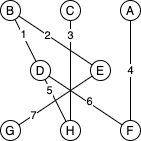
\includegraphics[width=0.9\textwidth]{figures/hypergraph_coloring/small_dependency_graph.drawio.png}
%         \caption{A depdendency graph for a simple 3-epoch computation}\label{fig:dependence-graph}
%     \end{subfigure}
%     \begin{subfigure}{0.24\textwidth}
%         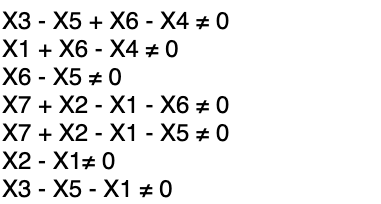
\includegraphics[width=0.9\textwidth]{figures/hypergraph_coloring/hypergraph_relations.drawio.png}
%         \caption{The path relations induced by the dependency graph}\label{fig:path-relations}
%     \end{subfigure}
%     \begin{subfigure}{0.24\textwidth}
%         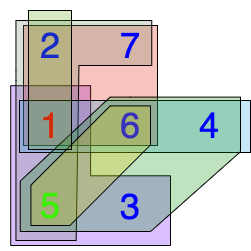
\includegraphics[width=0.9\textwidth]{figures/hypergraph_coloring/colored_dependency_hypergraph.drawio.png}
%         \caption{A minimal coloring of the hypergraph corresponding to the path relations}\label{fig:colored-hypergraph}
%     \end{subfigure}
%     \begin{subfigure}{0.24\textwidth}
%         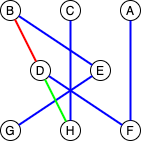
\includegraphics[width=0.9\textwidth]{figures/hypergraph_coloring/colored_dependency_graph.drawio.png}
%         \caption{The coloring applied to the original dependency graph. Edges with the same color correspond to the same rotation amount.}\label{fig:colored-dependence-graph}
%     \end{subfigure}
%     \vspace{-1em}
%     \caption{An example coloring the edges of a dependency graph to produce a good lane assignment}\label{fig:lane-assignment}
%     \Description{TODO: insert description}
% \end{figure*}

% \begin{algorithm}
%     \SetKwFunction{hypergraph}{MakeHypergraph}
%     \SetKwFunction{colorhg}{ColorHypergraph}
%     \SetKwFunction{makeilp}{FormulateILP}
%     \SetKwFunction{solveilp}{SolveILP}
%     \SetKwFunction{placelanes}{PlaceLanes}
%     \SetKwFunction{paths}{Paths}
%     \SetKwFunction{edges}{Edges}
%     \SetKwFunction{startepoch}{StartEpoch}
%     \SetKwFunction{endepoch}{EndEpoch}
%     \SetKwFunction{hyperdegree}{Hyperdegree}
%     \SetKwFunction{nextcol}{GetColor}

%     \SetKwProg{proc}{Procedure}{}{}
%     \SetKwProg{algo}{Algorithm}{}{}

%     \algo{\placelanes{deps}}{
%         $rels \gets \hypergraph{deps}$\;
%         $coloring \gets \colorhg(rels)$\;
%         $ilp \gets \makeilp{deps, rels, coloring}$\;
%         $placement \gets \solveilp{ilp}$\;
%         \Return{placement}\;
%     }

%     \proc{\hypergraph{deps}}{
%         $V\gets \edges{deps}$\;
%         $E_{hyper}\gets\emptyset$\;
%         \ForEach{$p \in \paths{deps}$}{
%             \If{\startepoch{p} = \endepoch{p}}{
%                 $E_{hyper}\gets E\cup \{\edges{p}\}$\;
%             }
%         }
%         \Return{V, $E_{hyper}$}
%     }
%     \proc{\colorhg{hypergraph}}{
%         $coloring \gets \emptyset$\;
%         \While{not fully colored}{
%             $e \gets\arg\min_{e'}\hyperdegree{e'}$\;
%             $coloring[e]\gets\nextcol{e, hypergraph}$\;
%         }
%         \Return{coloring}
%     }
%     \caption{Lane placement algorithm}\label{alg:lane-placement}
% \end{algorithm}

% Once the entire program is scheduled, each epoch produces a set of outputs which may feed into inputs of subsequent epochs.
% Since no rotation happens within an epoch, each input of an epoch must be on the same lane as the output of the epoch it eventually flows into.
% This creates a dependence between the output of one epoch with the output of a downstream epoch, in the sense that if these do not map to the same lane, we need to insert a rotation to line them up.
% % Once the entire program is scheduled, each epoch produces a set of outputs which may depend on outputs from previous epochs.
% % Each output is produced on a single lane, and whenever a pair of outputs with a dependence between them do not map to the same lane, we need to insert a rotation to get them to line up. \raghav{is this better?}

% % Scheduling the program in the way described above amounts to splitting it into a number of {\em epochs}, where each epoch consists of a set of subexpressions to compute. \milind{again ``phase'' vs ``stage''. Also, what's important here isn't that you have the phases -- what's important is that each phase generates output operands in particular lanes, and those operands might need to hook up to one or more input operands in other phases, which means that either the lanes need to be set so everything lines up right, or you need to add rotations.}
% For a program that is split into $k$ epochs, we can represent these dependencies in a $k$-partite graph, where each partition corresponds to a epoch and each vertex in a partition corresponds to a subexpression computed in that epoch.
% Figure~\ref{fig:dependence-graph} shows an example 3-partite dependence graph for a particular 3-epoch program, where the first epoch had three subexpressions in it, the second had two, and the third had three.
% To assign lanes to the subexpressions, we need to assign a number to each vertex in this dependence graph such that no two vertices in the same epoch get the same number.
% Unfortunately, a naive approach to this can have very poor results: consider, for example, placing B, D, and G on lane 1; C, E, and F on lane 2; and A and H on the lane 3.
% This particular placement requires one rotation each to line up B with E, A with F, and C with H, an additional two rotations to line up D with H and F, and a final rotation to line up E with G.
% In the worst case, this incurs six rotations.
% In the best case, if the vector schedule happens to pack the outputs of B and C together into the same vector, the $B\rightarrow E$ and $C\rightarrow H$ rotations are the same (since they are both a rotation of 1); similarly, if D and E are packed into the same vector, the $D\rightarrow F$ and $E\rightarrow G$ rotations are the same, requiring a total of four rotations to line everything up. 
% % This particular placement requires one rotation to line B up with E, an additional two rotations to line D up with H and F, respectively, and a final rotation to line up E with G, incurring a total of four rotations. 
% But we can do better: if we instead place B, E, and G on lane 1, A, D and F on lane 2, and C and H on lane 3, we can align the epochs with only two rotations: one to line up B and D, and one to line up D and H. 
% The goal of lane assignment (Algorithm~\ref{alg:lane-placement}) is to automatically determine that optimal placement.

% The heuristic approach is to place vertices on lanes while getting as many edges as possible to have the same rotation along them.
% It would be much easier to reason about this by assigning rotation values to edges instead of assigning lanes to vertices: a positive value on the edge represents rotating the value to the right before continuing the computation, a negative value represents rotating the value to the left, and a zero represents no rotation.
% But note that there is a subtlety we need to keep track of here: not every assignment of rotation values to edges comes from a consistent assignment of lanes to vertices. 

% There are three consistency requirements: If the same input value (which is in a particular lane) flows through different operations to the same output value (which is in a particular, possibly different, lane), then all the rotations along the two sequences of operations should eventually place the results on the same lane to generate the output. 
% On the other hand, if the same input value flows to two {\em different} outputs, then the rotations along those two paths {\em must} place the final results in different lanes. %\milind{does the preceding explanation of the consistency requirements make sense?} \milind{Maybe give an example of what an inconsistent rotation set looks like.}
% Dually, if two different input values flow to the same output, then both paths should still agree on which lane to place the output.
% %\raghav{That's the third constraint. I think being vague enough about `path' makes it okay?}
% For an example of an inconsistent assignment, consider the dependence graph in Figure~\ref{fig:dependence-graph}.
% If edges 5 and 6 both get assigned a value of 0, then $D$ must be on the same lane as both $H$ and $F$.
% This means that $H$ and $F$ must be on the same lane, which violates the first consistency constraint.
% %\raghav{I think the consistency requirements written above are too weak, but maybe its sufficient for intuition?}

% The consistency requirements can be reinterpreted as follows: for any path that starts and ends on the same epoch in the dependence graph, the {\em directed sum} of the rotation values along it should be zero if the path is a cycle, and nonzero otherwise.
% (In a directed sum, we assign a direction to each edge, and negate its value if we follow the edge backwards).
% Notice that this automatically enforces that two different paths between a pair of vertices should add up to the same value, since any two such paths also form a cycle by inverting one of them, and the cycle needs to add up to 0. 
% % Instead, we try to assign lanes in a way that minimizes the number of {\em distinct} rotations required for each vector (for example, if multiple pieces of data on the same vector are produced two lanes away from where they are consumed, we can rotate the vector a single time to get them both to line up).
% % In other words, given a $k$-partite graph with an integer associated to each vertex, we can assign to each edge the difference of its two endpoints, representing the rotation. 
% % To minimize the distinct numbers we have to assign to the edges, we'd like to be able to go backwards: in other words, we want to assign as few numbers as possible to all the edges such that ``integrating'' them gives a consistent assignment of numbers to the vertices.

% % This consistency constraint can be reworded as follows: For every path through the $k$-partite graph that starts and ends on the same partition, the directed sum of the edge weights along that path must be 0 if the path is a cycle, or nonzero otherwise.
% % (Notice that this automatically enforces the condition that two different paths between a pair of vertices on the same partition must add up to the same value, since concatenating one path with the reversal of the other produces a cycle, which must sum to 0).
% % \raghav{If only I could figure out a neat and tidy way to describe this whole process mathematically\dots}

% Iterating over all the paths in the graph yields a set of linear {\em path relations} as shown in Figure~\ref{fig:path-relations}, where initially all of the $X_i$s are unassigned.
% To assign a particular $X_i$, if it is part of a relation where it is the only unassigned variable, its value is fixed to be one that satisfies the relation; otherwise, it can be assigned freely.
% These constraints form a hypergraph like the one in Figure~\ref{fig:colored-hypergraph}, where the vertices $1,\dots, 7$ correspond to edges in Figure~\ref{fig:dependence-graph}, and each path relation becomes a hyperedge connecting the associated vertices.

% To find a consistent assignment of rotation values to edges we must color this hypergraph such that the last vertex to be colored on any hyperedge is given a distinct color from the rest of the vertices on the hyperedge (this is equivalent to producing a fresh value for the last $X_i$ to be assigned in a path relation, so it can freely be assigned to satisfy the relation).
% To minimize the number of distinct rotations needed, we would like to use as few colors as possible.
% This is relatively straightforward to do: At each step we pick the vertex that is part of as few ``free'' hyperedges as possible and assign it the next available color, until all the vertices have been colored.
% In the example shown in Figure~\ref{fig:colored-hypergraph}, we first assign to $X_3, X_4$, and $X_7$, (hyperdegree 2), then to $X_2$ and $X_6$ (hyperdegree 3), and then to $X_1$ and $X_5$ (hyperdegree 4).
% Since $X_1$ is the last vertex to be assigned in the relation $X_2 - X_1 \neq 0$, it must be given a color other than blue, so it gets red, and since $X_5$ is the last to be assigned in the relation $X_3 - X_5 - X_1 \neq 0$, it cannot be red or blue, so it gets green.

% Once the vertices of the hypergraph are colored, we can use it to color the edges of the original dependence graph, like in Figure~\ref{fig:colored-dependence-graph}. 
% Now, all that remains is getting actual rotation for each color. 
% This can be formulated as a simple integer program, with a variable $c_i$ for each color, a variable  $v_j$ for each node in the dependence graph, and a constraint for each edge $(v, v')$ colored $c$ to assert $v - v' == c$.
% The way we colored the hypergraph ensures that this integer program is always solvable, and the solution tells us exactly which vector lane each instruction should go on.